\documentclass[11pt,a4paper]{article}
\usepackage[margin=2.2cm]{geometry}
\usepackage{graphicx}
\usepackage{booktabs}
\usepackage{tabularx}
\usepackage{amsmath}
\usepackage{float}
\usepackage{caption}
\usepackage{xcolor}
\usepackage{enumitem}
\usepackage{fancyvrb}
\usepackage[hidelinks]{hyperref}

\setlength{\parskip}{0.5em}
\setlength{\parindent}{0pt}
\renewcommand{\arraystretch}{1.2}
\setlist{itemsep=2pt,topsep=2pt}

% placeholder for a screenshot that has not been added yet
\newcommand{\shot}[2]{%
  \IfFileExists{#1}{\includegraphics[width=#2]{#1}}{%
    \fbox{\parbox[c][4cm][c]{0.8\linewidth}{\centering\color{red}%
    Screenshot missing: \texttt{\detokenize{#1}}}}}}

% text the team still has to fill in
\newcommand{\todo}[1]{{\color{red}[TO FILL: #1]}}

\title{\textbf{4-bit Array Multiplier from RTL to GDSII}\\[4pt]
\large Digital VLSI Design: Assignment Report}
\author{Het Selarka (2024102031) \and Shrenil Patel (2024102066)}
\date{October 2026}

\begin{document}
\maketitle

\begin{center}
Repository:
\url{https://github.com/BMIrocks/4-bit-Array-Multiplier-from-RTL-to-GDSII}
\end{center}

\section*{Overview}

We designed a 4-bit $\times$ 4-bit unsigned array multiplier in Verilog (16 AND gates, 12 full
adders, input and output registers), verified it with an exhaustive testbench, synthesised it to
SkyWater SKY130 standard cells with Yosys, analysed its timing with OpenSTA, and took it through
place and route to a GDSII layout with LibreLane.

\textbf{Tools.} Instead of the IIC-OSIC-TOOLS image we used the official LibreLane 2.4.13 Docker
image (low disk space and a slow network made the 4\,GB image impractical). It contains the same
tools: Icarus Verilog 12.0, Yosys 0.46, OpenSTA 2.6.0, OpenROAD, Magic 8.3, Netgen and
KLayout 0.29, with the SKY130A PDK. All commands are listed in order in \texttt{README.md}.

%==================================================================
\section{Part A: RTL Design and Verification}

\texttt{rtl/full\_adder.v} describes one full adder with two \texttt{assign} statements
($s = a \oplus b \oplus c_{in}$, $c_{out} = ab + ac_{in} + bc_{in}$).
\texttt{rtl/mult\_array.v} registers $a$ and $b$, forms the 16 partial product bits
$a_jb_i$, adds them in three rows of four full adders (12 instances) exactly as in the
equations of Section 2 of the assignment, and registers the 8-bit product $p$. All 16
flip-flops have an asynchronous active-low reset.

\begin{figure}[H]
  \centering
  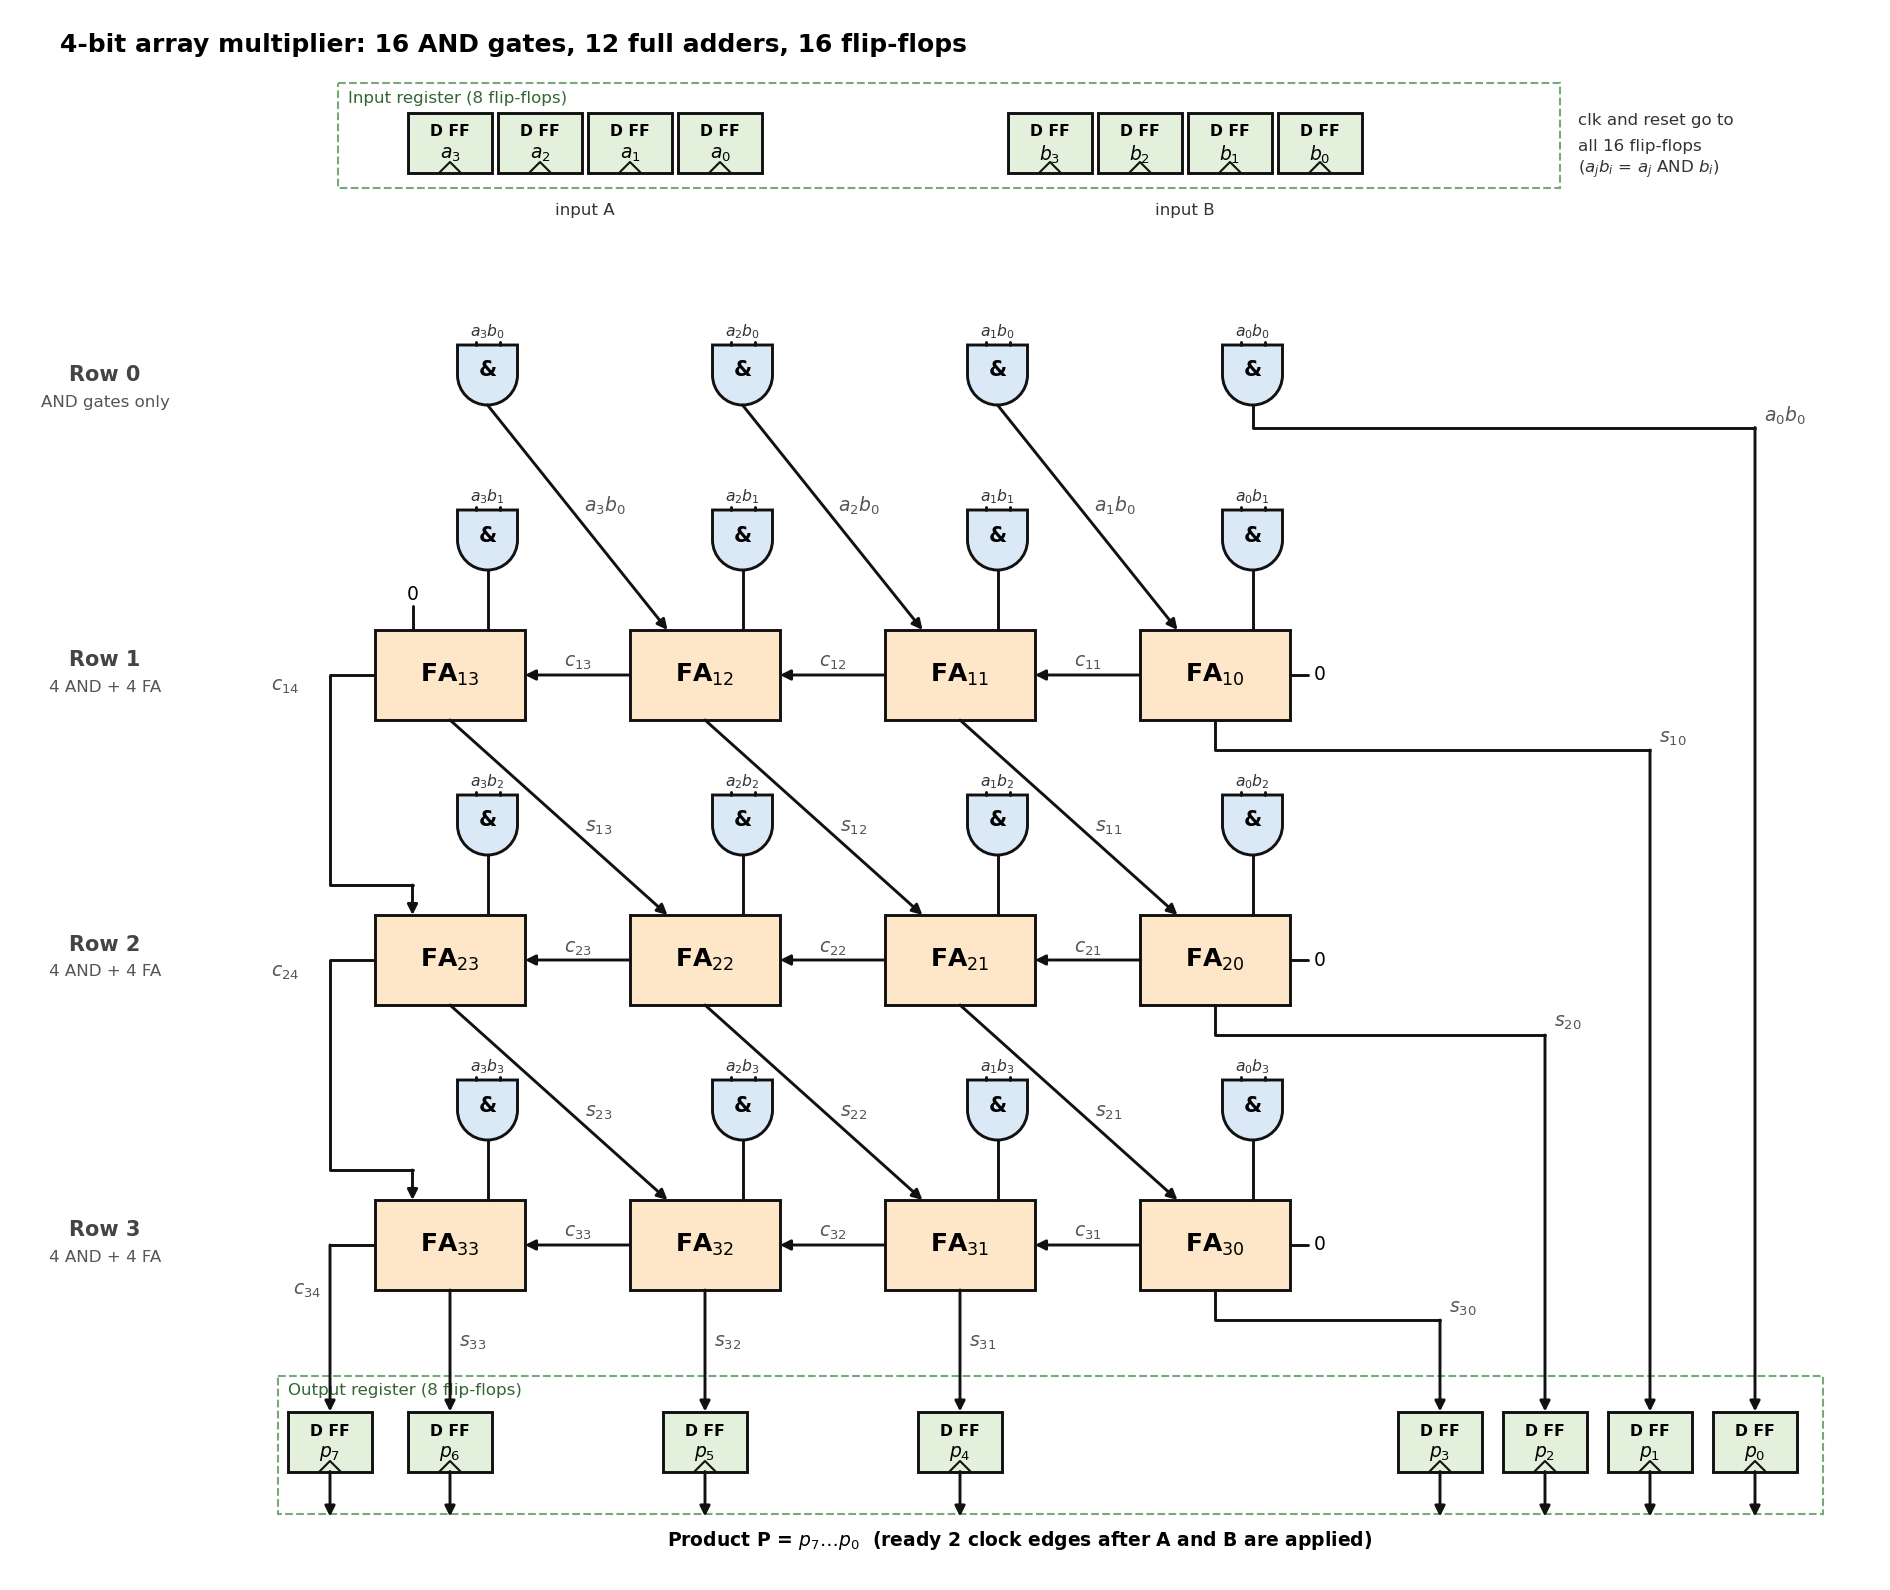
\includegraphics[width=0.92\linewidth]{block_diagram.png}
  \caption{Block diagram: 8 input flip-flops, 16 AND gates, 12 full adders FA$_{10}$ to
  FA$_{33}$ and 8 output flip-flops.}
\end{figure}

\subsection*{Verification}

The testbench \texttt{tb/tb\_mult.v} uses a 10\,ns clock, holds reset low for 2 cycles, applies
all 256 input pairs and checks every product after the 2-cycle latency.

\begin{Verbatim}[frame=single,fontsize=\small]
$ iverilog -g2012 -o sim tb/tb_mult.v rtl/full_adder.v rtl/mult_array.v && vvp sim
PASS: 256 vectors checked, 0 errors
\end{Verbatim}

\textbf{Fault test.} With the sum in \texttt{full\_adder.v} changed to $a \oplus b$ the same
testbench prints:
\begin{Verbatim}[frame=single,fontsize=\small]
FAIL: 256 vectors checked, 95 errors
\end{Verbatim}
so it does detect a wrong design. The first mismatches it printed were $a = 3, b = 3$ (expected 9,
got 5) and $a = 3, b = 6$ (expected 18, got 10). For $3 \times 3$ both $a_0b_1$ and $a_1b_0$ are 1,
so FA$_{10}$ produces a carry into FA$_{11}$; the broken adder drops its carry-in from the sum, so
this is the first pair in the test order where the fault becomes visible. A bit-level model of the
array confirms that the 95 failing pairs are exactly the pairs in which at least one adder receives
a carry-in of 1; the other 161 pairs never use a carry-in and still give the right product. The correct
equation was restored afterwards and the testbench printed PASS again.

\subsection*{Hand-worked example}

Het's roll number ends in 1, so $A = 1 + 5 = 6$ and $B = 7$.

\begin{figure}[H]
  \centering
  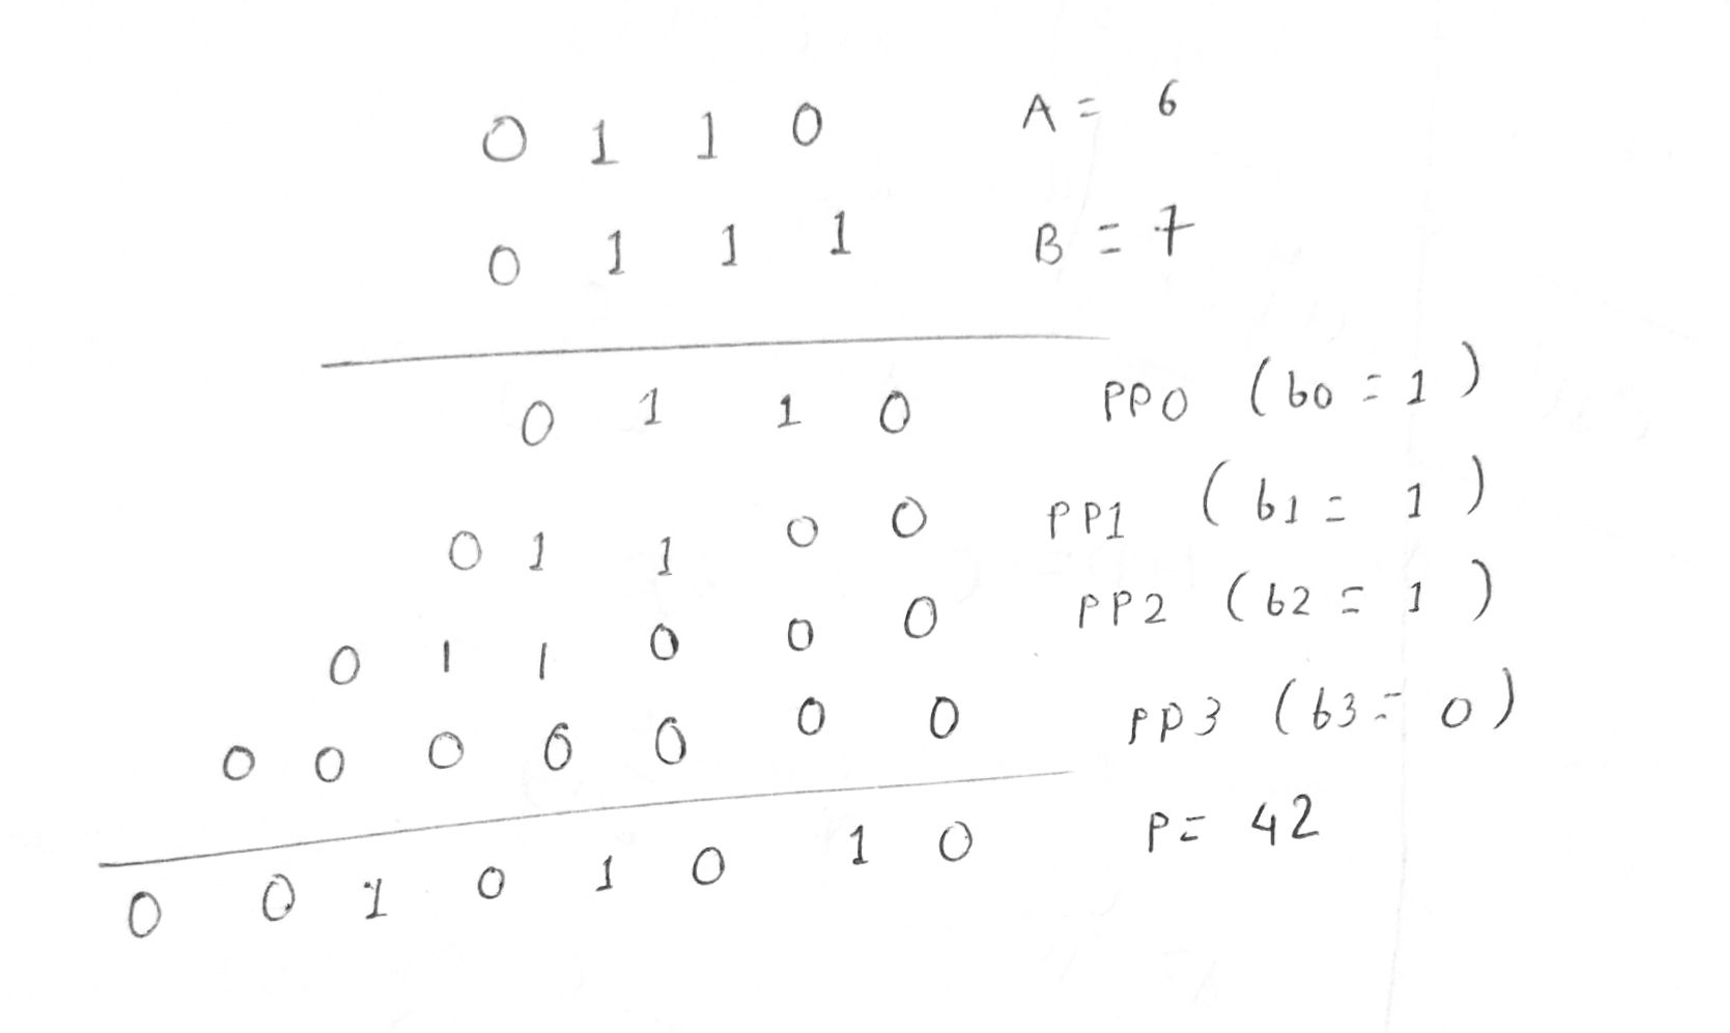
\includegraphics[width=0.7\linewidth]{hand_example.png}
  \caption{Hand-worked example: $6 \times 7 = 42$ ($0110 \times 0111 = 0010\,1010$), with the four
  shifted partial products PP0 to PP3.}
\end{figure}

The same multiplication through the rows of the array:

\begin{center}
\small
\begin{tabular}{@{}clll@{}}
\toprule
Row & Adds & Sum, carry & Product bit \\
\midrule
0 & PP0 = 0110 & -- & $p_0 = 0$ \\
1 & 0110 + 0011 & 1001, 0 & $p_1 = 1$ \\
2 & 0110 + 0100 & 1010, 0 & $p_2 = 0$ \\
3 & 0000 + 0101 & 0101, 0 & $p_3 = 1$ \\
\bottomrule
\end{tabular}
\end{center}

Each row keeps its lowest sum bit as a product bit and passes the other three sum bits and its
carry down. Row 3 also gives $p_7..p_4 = 0010$, so $P = 0010\,1010 = 42$.

\subsection*{Waveform}

\begin{figure}[H]
  \centering
  \shot{waveform_6x7.png}{0.95\linewidth}
  \caption{$A = 6$, $B = 7$ is applied at 2090\,ns, captured into the input register at the
  rising edge at 2095\,ns (marker A) and $p$ changes from 36 to 42 at the next rising edge,
  2105\,ns (marker B): a latency of 2 clock edges.}
\end{figure}

\textbf{Why $p$ usually shows the previous product.} In the waveform $p$ most of the time looks like
$A \times (B-1)$ (for example $a = 6$, $b = 5$ next to $p = 24$). This is the 2-cycle latency, not an
error. Each input pair is held for 20\,ns; its product appears 15\,ns after it is applied, so for
the first 15\,ns $p$ still holds the product of the previous pair, and only in the last 5\,ns do
$a$, $b$ and $p$ belong to the same multiplication. We checked all 239 changes of $p$ in the
waveform: each equals $a \times b$ of the inputs captured one clock edge earlier.

%==================================================================
\section{Part B: Logic Synthesis with Yosys}

\texttt{synth/synth.tcl} reads the RTL, synthesises and flattens it, maps the flip-flops
(\texttt{dfflibmap}) and the logic (\texttt{abc}) to SKY130 cells, removes unused wires, and
writes the cell report and the gate-level netlist, using the typical-corner cell library
(25\,\textdegree C, 1.80\,V).

\begin{table}[H]
\centering
\begin{tabularx}{0.9\linewidth}{@{}lX@{}}
\toprule
Metric & Value \\
\midrule
Total number of cells & 65 \\
Number of flip-flops & 16 (dfrtp\_1) \\
Total cell area & 751.97\,\textmu m$^2$ \\
Flip-flop area & $16 \times 25.024 = 400.38$\,\textmu m$^2$ \\
Flip-flop area (\% of total) & 53.24\,\% \\
3 most-used cell types & dfrtp\_1: 16, nand2\_1: 7, then a tie at 5 each:
  a21oi\_1, nor2\_1, xnor2\_1, xor2\_1 \\
Netlist simulation result & \texttt{PASS: 256 vectors checked, 0 errors} \\
\bottomrule
\end{tabularx}
\caption{Part B results.}
\end{table}

The other cells are maj3 (4), a22oi (3), and4 (3), and2 (2), nor3 (2), xnor3 (2),
lpflow\_isobufsrc (2) and one each of a211oi, nand3, o21a and o21ai.

\textbf{Problem found in the netlist simulation.} The first gate-level run printed
\texttt{FAIL: 256 vectors checked, 239 errors}; every wrong value was the product of the previous
input pair. With \texttt{-DUNIT\_DELAY=\#1} each flip-flop model has a 1\,ns clock-to-output delay,
and the testbench originally checked $p$ exactly 1\,ns after the clock edge, at the same instant as
the update. We moved the check to 4\,ns after the edge (still before the inputs change at the
next falling edge). After that, RTL and netlist simulation both pass and the fault test still
fails as it should. The design itself was not changed.

\begin{table}[H]
\centering
\small
\begin{tabular}{@{}lll@{}}
\toprule
 & RTL simulation (Part A) & Gate-level simulation (Part B) \\
\midrule
Design & \texttt{full\_adder.v}, \texttt{mult\_array.v} & \texttt{mult\_array\_netlist.v} (65 SKY130 cells) \\
Testbench & \texttt{tb\_mult.v} & \texttt{tb\_mult.v} (same file) \\
Cell models & -- & \texttt{primitives.v}, \texttt{sky130\_fd\_sc\_hd.v} \\
Vectors checked & 256 & 256 \\
Errors & 0 & 0 \\
Result & PASS & PASS \\
\bottomrule
\end{tabular}
\caption{The same exhaustive testbench passes on the RTL and on the synthesised netlist, so
synthesis did not change the behaviour, the latency or the reset.}
\end{table}

%==================================================================
\section{Part C: Static Timing Analysis with OpenSTA}

\texttt{sta/sta.tcl} reads the library and the netlist, creates the clock, sets 1\,ns input and
output delays and reports the worst setup slack and the critical path. The period is a variable
(10\,ns by default).

\begin{itemize}
  \item At $T = 10$\,ns: WNS $= 7.324$\,ns, so $T_{min} = 10 - 7.324 = 2.676$\,ns and
        $F_{max} = 1000 / 2.676 = 373.7$\,MHz.
  \item At $T = 2.68$\,ns ($T_{min}$ rounded): worst slack $= 0.004$\,ns $\approx 0$.
\end{itemize}

\begin{table}[H]
\centering
\begin{tabularx}{0.9\linewidth}{@{}lX@{}}
\toprule
Metric & Value \\
\midrule
Worst slack at $T = 10$\,ns & 7.324\,ns \\
$T_{min}$ & 2.676\,ns \\
$F_{max}$ & 373.7\,MHz \\
Slack at $T = T_{min}$ (2.68\,ns) & 0.004\,ns \\
Critical path start point & input register flip-flop of $b_0$ \\
Critical path end point & output register flip-flop of $p_6$ \\
Number of cells on the critical path & 9 (launching flip-flop + 8 logic gates) \\
Latency $= 2 \times T_{min}$ & 5.35\,ns \\
Throughput & 373.7 million results per second \\
\bottomrule
\end{tabularx}
\caption{Part C results (typical corner, tt\_025C\_1v80).}
\end{table}

\begin{table}[H]
\centering
\small
\begin{tabular}{@{}rllrrl@{}}
\toprule
\# & Cell & Function & Delay (ns) & Arrival (ns) & Full adder \\
\midrule
1 & dfrtp\_1 & $b_0$ flip-flop, clock to Q & 0.386 & 0.386 & -- \\
2 & and4\_1 & $a_0b_1 \cdot a_1b_0$ = carry of FA$_{10}$ & 0.251 & 0.638 & FA$_{10}$ \\
3 & nor3\_1 & carry of FA$_{11}$ (part 1) & 0.217 & 0.855 & FA$_{11}$ \\
4 & o21ai\_0 & carry of FA$_{11}$ (part 2) & 0.173 & 1.028 & FA$_{11}$ \\
5 & maj3\_1 & carry of FA$_{12}$ & 0.404 & 1.431 & FA$_{12}$ \\
6 & xnor2\_1 & sum of FA$_{13}$ & 0.166 & 1.598 & FA$_{13}$ \\
7 & maj3\_1 & carry of FA$_{22}$ & 0.389 & 1.987 & FA$_{22}$ \\
8 & maj3\_1 & carry of FA$_{23}$ & 0.380 & 2.367 & FA$_{23}$ \\
9 & xnor3\_1 & sum of FA$_{33}$ $= p_6$ & 0.175 & 2.542 & FA$_{33}$ \\
\midrule
 & & setup time of the $p_6$ flip-flop & 0.134 & 2.676 & \\
\bottomrule
\end{tabular}
\caption{Cells on the critical path (from \texttt{sta/mult\_array\_timing.rpt}). Each gate was
matched to its full adder from its inputs in the netlist.}
\end{table}

All 8 logic gates come from full adders. They cover 7 full adder stages
(FA$_{10} \rightarrow$ FA$_{11} \rightarrow$ FA$_{12} \rightarrow$ FA$_{13} \rightarrow$ FA$_{22}
\rightarrow$ FA$_{23} \rightarrow$ FA$_{33}$) against the estimate of about $2N = 8$.

%==================================================================
\section{Part D: Physical Design with LibreLane}

\texttt{pnr/config.json} sets the design name, the two Verilog files, the clock port, a fixed
$150 \times 150$\,\textmu m die and the clock period. The first period was
$1.2 \times 2.676 = 3.21$\,ns rounded up to 3.5\,ns.

LibreLane signs off timing at three corners: typical (25\,\textdegree C, 1.80\,V), slow
(100\,\textdegree C, 1.60\,V) and fast ($-40$\,\textdegree C, 1.95\,V). We used the worst of them
(\texttt{timing\_\_setup\_\_ws}, always the slow corner) for the ``setup slack $\geq 0$'' rule and
raised the period by 0.5\,ns after each failing run:

\begin{table}[H]
\centering
\small
\begin{tabular}{@{}cccccc@{}}
\toprule
Run & CLOCK\_PERIOD (ns) & Slack, worst corner (ns) & Slack, typical (ns) & DRC & LVS \\
\midrule
1 & 3.5 & $-1.617$ & 0.808 & 0 & 0 \\
2 & 4.0 & $-1.107$ & 1.257 & 0 & 0 \\
3 & 4.5 & $-0.638$ & 1.797 & 0 & 0 \\
4 & 5.0 & $-0.106$ & 2.309 & 0 & 0 \\
5 & 5.5 & $\phantom{-}0.120$ & 2.693 & 0 & 0 \\
\bottomrule
\end{tabular}
\caption{All LibreLane runs. Run 5 is the final one.}
\end{table}

\begin{table}[H]
\centering
\begin{tabularx}{0.95\linewidth}{@{}lX@{}}
\toprule
Metric & Value \\
\midrule
CLOCK\_PERIOD used & 5.5\,ns \\
Number of runs needed & 5 \\
Core area & 17\,759.5\,\textmu m$^2$ (die $150 \times 150 = 22\,500$\,\textmu m$^2$) \\
Cells after synthesis (Part B) & 65 \\
Cells after place and route & 340 (plus 1\,559 fill and decap cells, 1\,899 in total) \\
Kinds of cells added & tap cells (245), buffers (24: 4 clock tree, 9 input, 8 output, 3 fanout),
  decap cells (1\,295), fill cells (264) \\
Wirelength & 2\,571\,\textmu m \\
Setup slack & 0.120\,ns (worst corner); 2.693\,ns (typical corner) \\
Post-route $F_{max}$ & $1000/(5.5-0.120) = 185.9$\,MHz (worst corner);
  $1000/(5.5-2.693) = 356.3$\,MHz (typical) \\
$F_{max}$ from Part C & 373.7\,MHz (typical corner) \\
DRC errors & 0 (Magic, KLayout and router) \\
LVS errors & 0 \\
\bottomrule
\end{tabularx}
\caption{Part D results. Antenna, max slew, max capacitance and hold checks also pass.}
\end{table}

\begin{table}[H]
\centering
\small
\begin{tabular}{@{}lrl@{}}
\toprule
Kind & Count & Cells \\
\midrule
Flip-flops & 16 & dfrtp\_1 (9), dfrtp\_2 (2), dfrtp\_4 (5); some upsized for timing \\
Logic gates & 55 & a21o, and3, xnor2, nand2, \ldots \\
Tap cells & 245 & tapvpwrvgnd\_1 \\
Clock tree buffers & 4 & clkbuf\_16 (3: root and two branches), clkbuf\_4 (1, clock load) \\
Input buffers & 9 & one per input pin except clk: clkbuf\_1 (8), buf\_1 (1) \\
Output buffers & 8 & one per product bit: buf\_2 \\
Fanout buffers & 3 & buf\_2 (2), clkbuf\_4 (1): split heavily loaded nets \\
\midrule
Counted in \texttt{instance\_\_count} & 340 & \\
\midrule
Decap cells & 1\,295 & decap\_3/4/6/8 (391), decap\_12 (904) \\
Fill cells & 264 & fill\_1 (219), fill\_2 (45) \\
\midrule
All cells in the layout & 1\,899 & \\
\bottomrule
\end{tabular}
\caption{Cells in the final layout. LibreLane's own synthesis gives 71 cells (16 flip-flops and
55 gates); everything else was added by the flow.}
\end{table}

\begin{figure}[H]
  \centering
  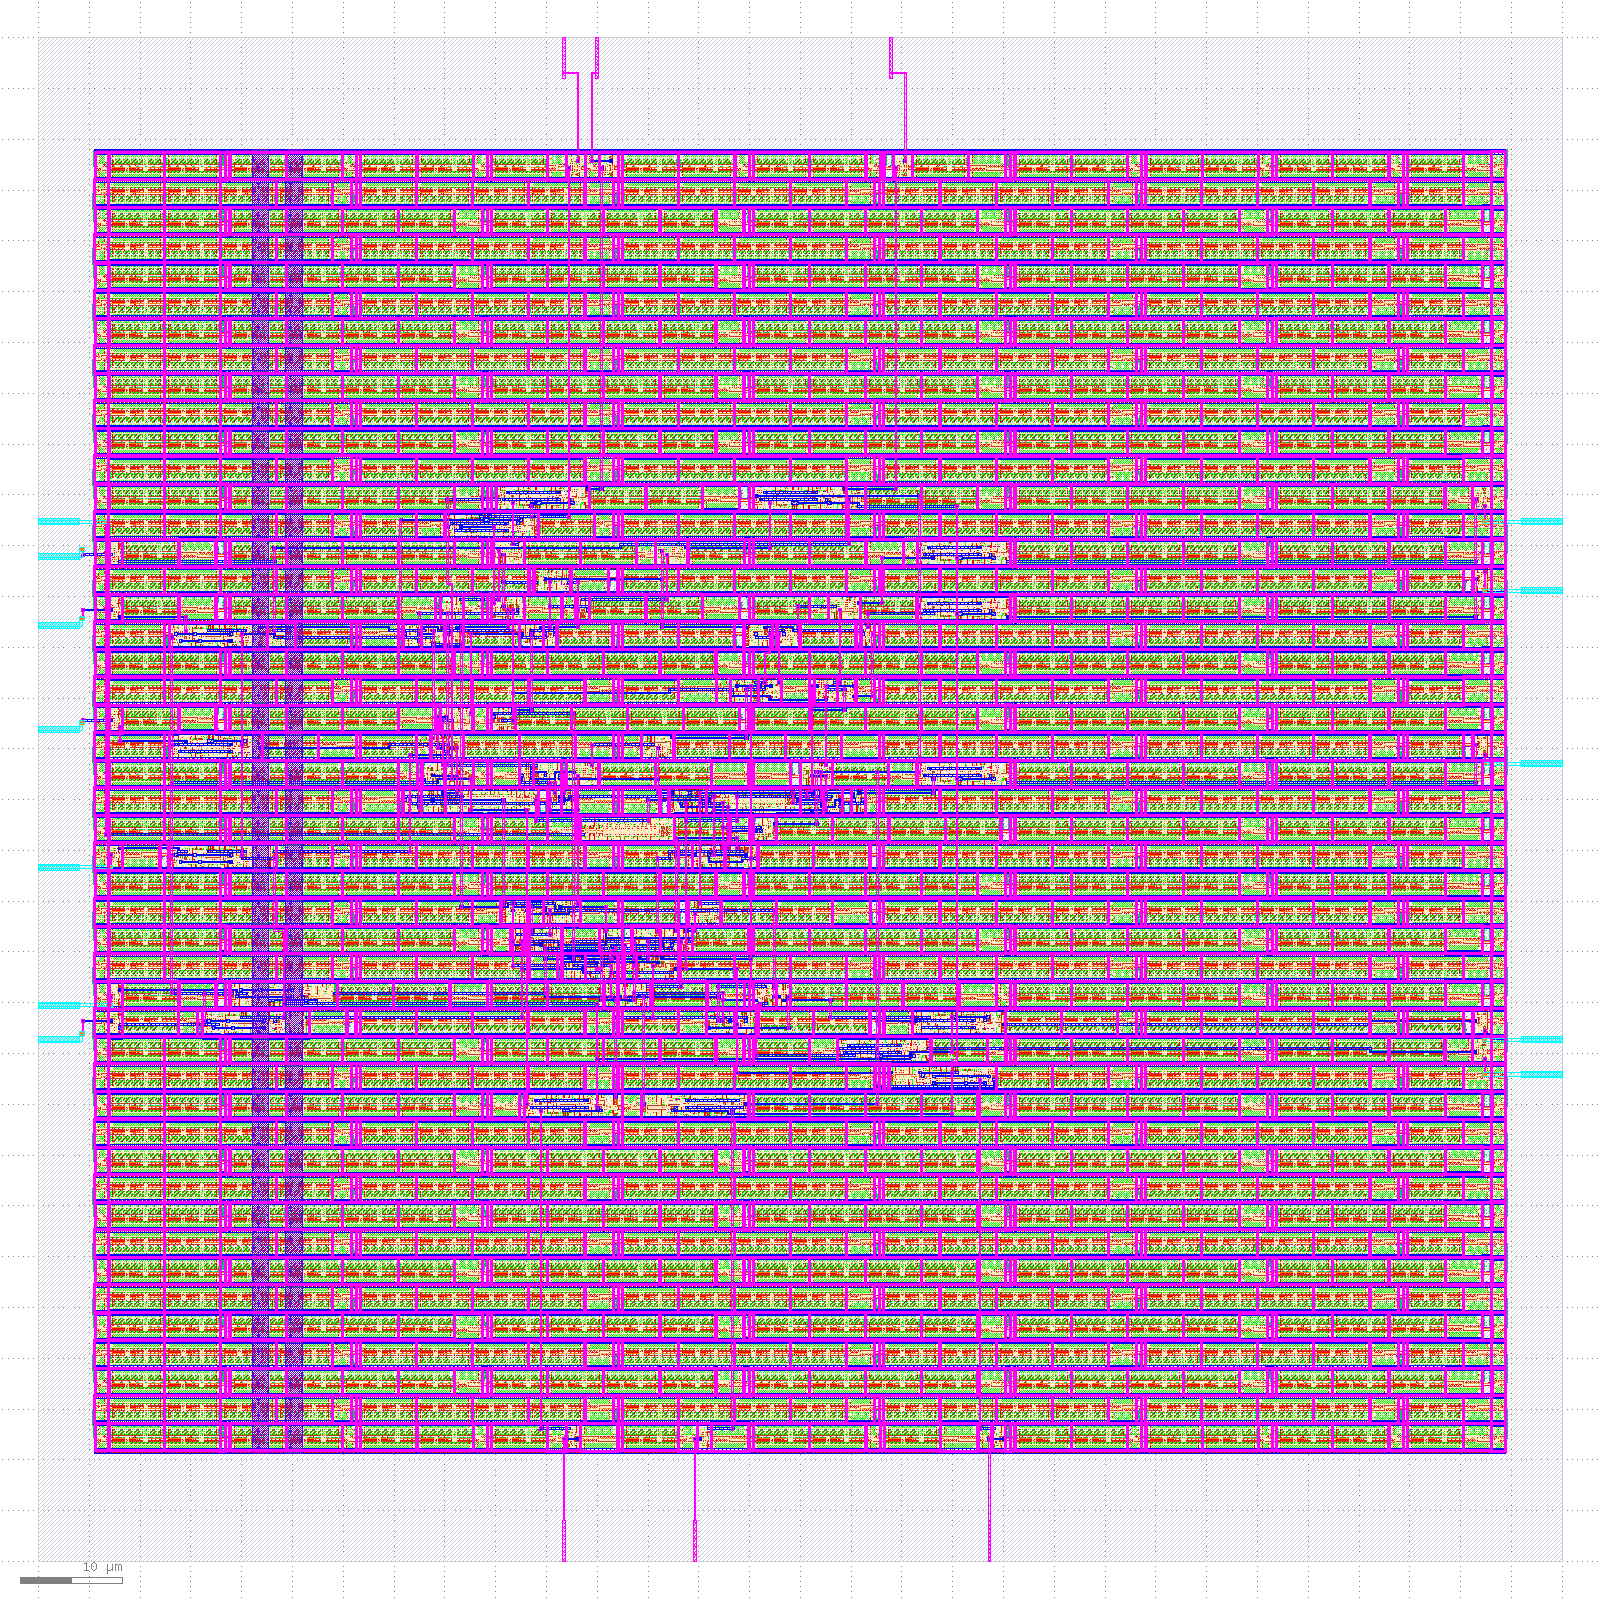
\includegraphics[width=0.48\linewidth]{layout_full_die.png}\hfill
  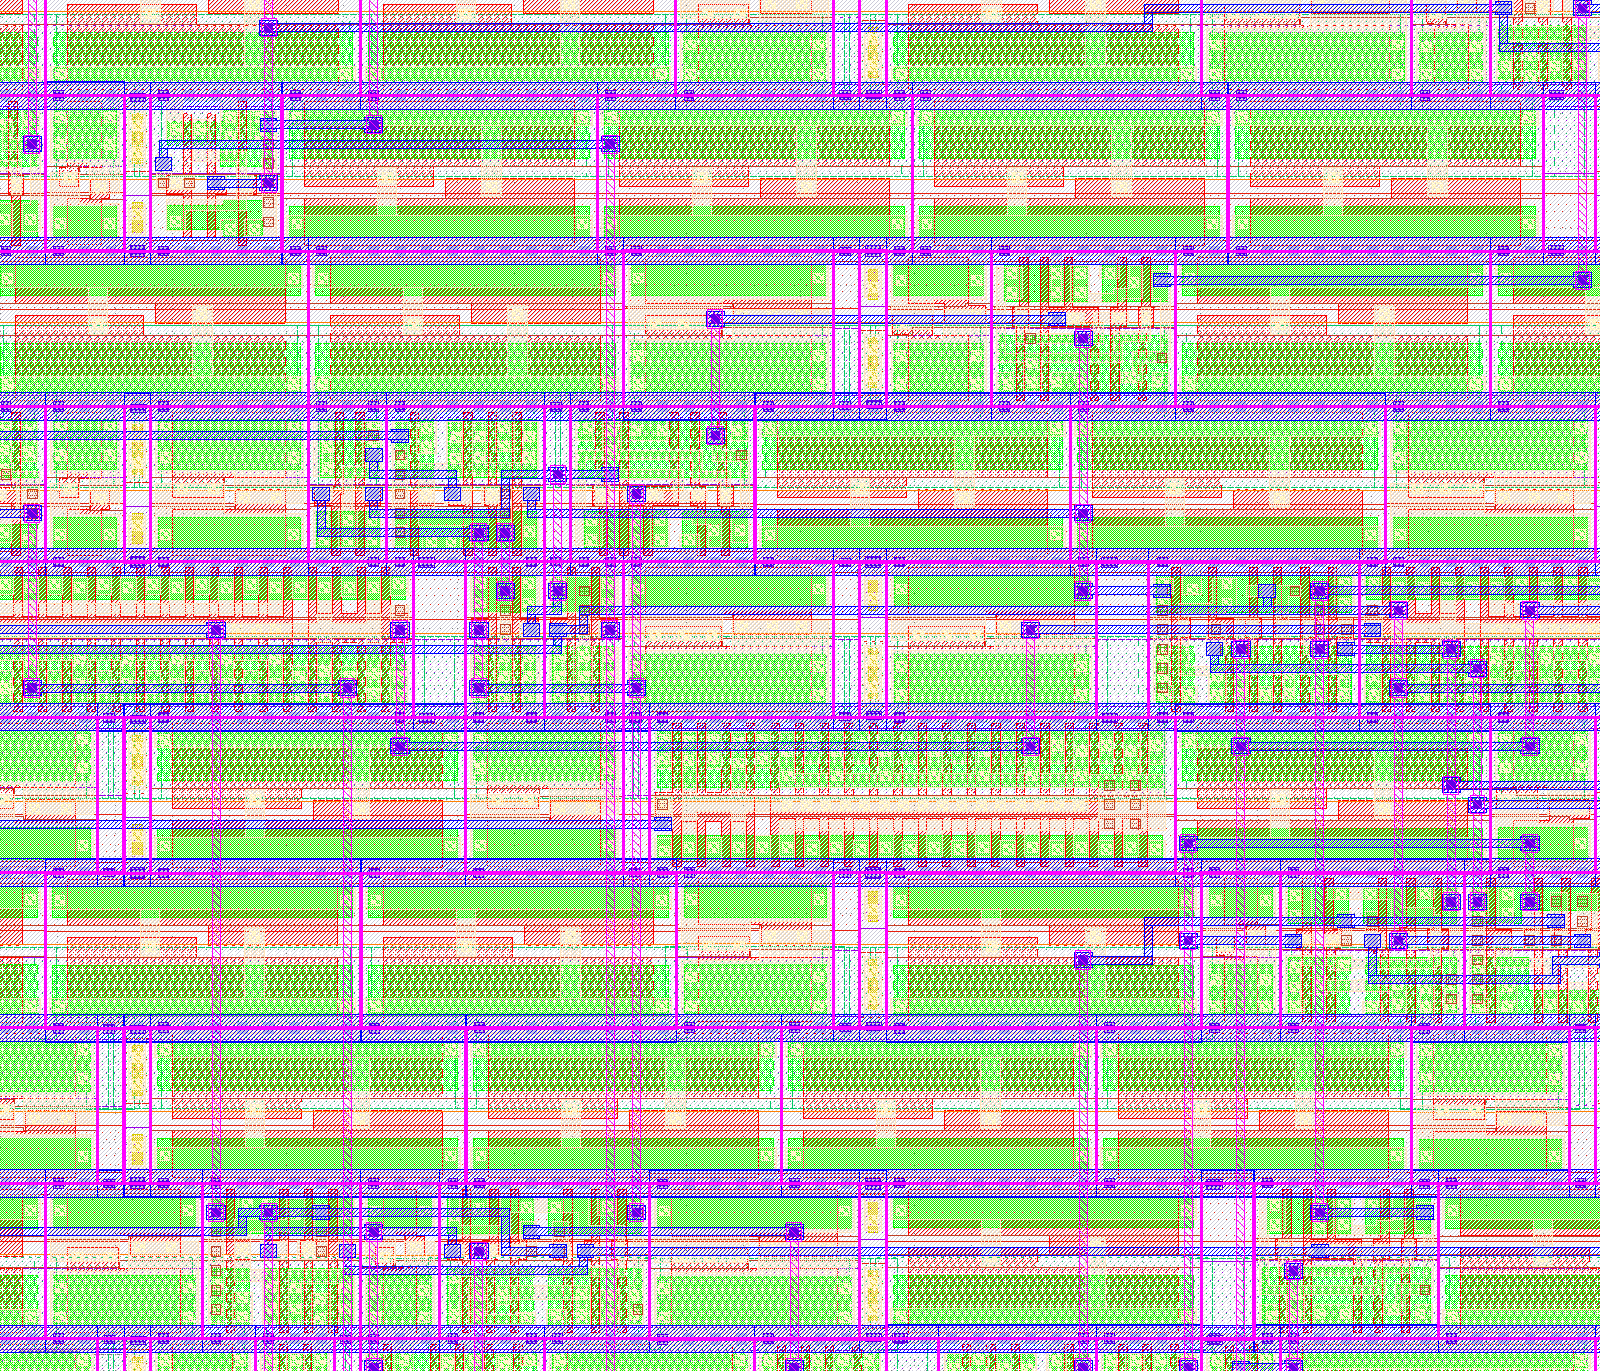
\includegraphics[width=0.48\linewidth]{layout_zoom.png}
  \caption{Final layout in KLayout (net name labels hidden). Left: the whole
  $150 \times 150$\,\textmu m die with the cell rows, power grid and pins on all four sides.
  Right: zoomed view of the logic with standard cell rows, metal wires and vias.}
\end{figure}

%==================================================================
\section{Answers to the Questions}

\textbf{1. Logic cells after synthesis.}
Synthesis produced 65 cells, of which 16 are flip-flops, so the logic is $65 - 16 = 49$ cells,
not $16 + 12 = 28$. A full adder is not one library cell here: \texttt{-flatten} removes the
full adder boundaries and ABC rebuilds the whole network from the gates it finds cheapest. ABC
cannot use the library full adder (\texttt{fa\_1}) because it has two outputs, so each adder
becomes several cells: a carry needs a maj3 or two AND-OR-INVERT gates, and a sum needs an xnor3
or two xor2/xnor2 gates. In the other direction many AND gates disappear because they are
merged into complex gates (and4, a21oi, a22oi), and the first adder in each row has carry-in 0,
so it shrinks to a half adder. The two effects together give 49 cells.

\textbf{2. Critical path.}
The critical path starts at the input register flip-flop of $b_0$ and ends at the output register
flip-flop of $p_6$. It has 9 cells: the launching flip-flop and 8 logic gates (and4, nor3, o21ai,
maj3, xnor2, maj3, maj3, xnor3), with an arrival time of 2.542\,ns plus 0.134\,ns setup time
$= 2.676\,\text{ns} = T_{min}$. The gates run through 7 full adder stages: the whole carry chain
of row 1 (FA$_{10}$ to FA$_{13}$), the carry chain of row 2 (FA$_{22}$, FA$_{23}$) and the top sum
of row 3 (FA$_{33}$). That is close to the estimate of $2N = 8$ full adder delays. It is one
stage shorter because the first adder of row 1 has carry-in 0 and was merged with its AND gates
into one and4 cell, and each stage costs only one or two gates.

\textbf{3. Flip-flop area.}
Flip-flops take 400.38 of 751.97\,\textmu m$^2$, which is 53.24\,\% of the total cell area. One
dfrtp\_1 flip-flop (25.02\,\textmu m$^2$) is about 6.7 times the size of a nand2\_1
(3.75\,\textmu m$^2$), because it contains two latches, a clock buffer and reset logic. The design
needs 16 of them (8 input, 8 output bits) but only 49 small logic gates, so the registers
dominate. The number of flip-flops grows only linearly with $N$ ($4N$) while the array grows
with $N^2$, so in a larger multiplier this percentage would be much smaller.

\textbf{4. Post-route $F_{max}$.}
At the typical corner (the one used in Part C) the post-route $F_{max}$ is 356.3\,MHz against
373.7\,MHz before layout, about 5\,\% lower. Part C had ideal wires and an ideal clock. After
routing every net has real resistance and capacitance extracted from the layout, so gates drive
heavier loads and switch more slowly; the clock reaches the flip-flops through a buffer tree
with some skew; the flow also adds a clock uncertainty margin of 0.25\,ns and a 0.15\,ns clock
transition to its constraints, which Part C did not have; and LibreLane's own synthesis
(71 cells) and resizing give a slightly different critical path. The 185.9\,MHz at the worst corner is lower mainly because transistors are much
slower at 100\,\textdegree C and 1.60\,V; the chip must work there too, which is why the period
had to be raised to 5.5\,ns. The flow added tap cells (245), which tie the n-well and substrate
to the supply rails at regular intervals to prevent latch-up; clock tree buffers (4), which drive
the clock to all 16 flip-flops with low skew; input and output buffers (17), one on every pin
except the clock, which give each pin a strong, known driver or load; fanout buffers (3), which
split nets that drive too many gates; decap cells (1\,295), small capacitors that keep
the supply voltage steady when many gates switch at once; and fill cells (264), which close the
gaps so the wells and power rails in every row are continuous.

\textbf{5. DRC and LVS.}
DRC (design rule check) verifies that the layout geometry obeys the foundry's rules: minimum
widths and spacings of every layer, enclosure of contacts and vias, density and antenna rules.
LVS (layout versus schematic) extracts the transistors and connections from the layout and
checks that they form exactly the same circuit as the netlist. Both must pass before
manufacturing: a DRC violation means the shapes may not be manufactured reliably (for example
shorts or breaks between wires, and low yield), while an LVS mismatch means the chip would be
made correctly but would be a different circuit from the one that was designed and verified. Our
final layout has 0 DRC errors (Magic and KLayout) and 0 LVS errors (Netgen).

\textbf{6. Scaling to 8 bits.}
Using the formulas of Section 2 with $N = 8$ instead of $N = 4$:
\begin{itemize}
  \item Full adders: $N(N-1) = 8 \times 7 = 56$ instead of $4 \times 3 = 12$, about 4.7 times
        more. AND gates: $N^2 = 64$ instead of 16, and flip-flops $4N = 32$ instead of 16.
  \item Critical path: about $2N = 16$ full adder delays instead of 8, i.e. twice as long.
\end{itemize}
From Part C, the logic part of our path is $T_{min} - t_{clk\to Q} - t_{setup} =
2.676 - 0.386 - 0.134 = 2.156$\,ns. Doubling it gives
$T_{min,8} \approx 2 \times 2.156 + 0.386 + 0.134 = 4.83$\,ns, i.e. $F_{max} \approx 207$\,MHz.
As a cross-check, our measured path had $2N - 1 = 7$ stages at about $2.156/7 = 0.31$\,ns each;
for $N = 8$ that is 15 stages, $15 \times 0.31 + 0.52 = 5.14$\,ns ($\approx 195$\,MHz). So the area
grows about with $N^2$ while the delay only grows about linearly with $N$.

%==================================================================
\section{Team Contributions}

\begin{table}[H]
\centering
\begin{tabularx}{\linewidth}{@{}p{0.2\linewidth}p{0.16\linewidth}X@{}}
\toprule
Part & Done by & Work \\
\midrule
A: RTL design and verification & Het Selarka & \texttt{full\_adder.v}, \texttt{mult\_array.v}
  (registers, partial products, the three adder rows), \texttt{tb\_mult.v}, fault test, hand-worked
  $6 \times 7$ example, waveform and latency explanation, block diagram. \\
B: Logic synthesis & Het Selarka & \texttt{synth.tcl}, synthesis run, Part B table, gate-level
  simulation and the testbench timing fix, Questions 1 and 3. \\
C: Static timing analysis & Shrenil Patel & \texttt{sta.tcl}, runs at $T = 10$\,ns and
  $T = T_{min}$, Part C table, critical path matched to the full adders, Questions 2 and 6. \\
D: Physical design & Shrenil Patel & \texttt{config.json}, the five LibreLane runs to timing
  closure, DRC/LVS checks, Part D table from \texttt{metrics.json}, post-route $F_{max}$,
  analysis of the added cells, layout screenshots, Questions 4 and 5. \\
Report & Both & Het: Parts A and B, Questions 1 and 3, README. Shrenil: Parts C and D,
  Questions 2, 4, 5 and 6. Both of us reviewed the final version. \\
\bottomrule
\end{tabularx}
\caption{Contributions by part.}
\end{table}

%==================================================================
\section{Conclusion}

The multiplier is correct at every level we could check: the exhaustive testbench passes on the
RTL and on the synthesised netlist, and a deliberately broken full adder is caught (95 errors).
Synthesis gives 65 cells and 751.97\,\textmu m$^2$, more than half of it flip-flops. Before layout
the design runs at up to 373.7\,MHz at the typical corner, limited by a path through seven full
adder stages from $b_0$ to $p_6$. After place and route the layout is DRC and LVS clean on a
$150 \times 150$\,\textmu m die; it meets timing at all corners with a 5.5\,ns clock and reaches
356.3\,MHz at the typical corner. The main lesson for us was that the frequency a design can be
signed off at depends far more on the slow process corner than on the wires the layout adds.

%==================================================================
\section{Use of AI Tools}

We wrote the RTL, the testbench and the synthesis script, ran the simulations and the fault test,
and worked out the hand example ourselves. We used an AI assistant for the Docker setup,
the first versions of \texttt{sta.tcl} and \texttt{config.json}, the LibreLane runs, debugging the
gate-level simulation, the diagrams and drafting this report. We checked all results against the
tool reports and can explain every part of the submission.

%==================================================================
\section*{References}

\begin{enumerate}[label={[\arabic*]}]
  \item N. Weste and D. Harris, \emph{CMOS VLSI Design: A Circuits and Systems Perspective},
        4th ed., Pearson, ch.~11.
  \item J. Rabaey, A. Chandrakasan and B. Nikoli\'c, \emph{Digital Integrated Circuits: A Design
        Perspective}, 2nd ed., Pearson.
  \item SkyWater SKY130 PDK documentation, \url{https://skywater-pdk.readthedocs.io}
  \item Yosys manual, \url{https://yosyshq.readthedocs.io/projects/yosys}
  \item OpenSTA, \url{https://github.com/parallaxsw/OpenSTA}
  \item LibreLane, \url{https://github.com/librelane/librelane}
  \item KLayout, \url{https://www.klayout.de}
\end{enumerate}

\end{document}
